% !TEX TS–program = pdflatexmk
% !TeX program used: pdftex

% \documentclass[12pt, aspectratio=169]{beamer}
\documentclass[12pt,aspectratio=169, handout]{beamer}
\usepackage[utf8]{inputenc}
\usepackage[T1]{fontenc}
\usepackage{url}
\usepackage{graphicx}
\usepackage{subcaption}

\usepackage{amsmath, amsfonts, amssymb}
\usepackage{mathtools}

% \usetheme{Madrid}
% \usetheme{Marburg}
% \usetheme{Frankfurt}
\usetheme{Berlin}
% \useoutertheme{split}
% \setbeamertemplate{navigation symbols}{}
% \usepackage[orientation=landscape,size=custom,width=16,height=9,scale=0.5,debug]{beamerposter} 
%\usepackage{enumitem}
\usepackage{ragged2e}
\usepackage{color}
\let\olditem\item
\renewcommand\item{\olditem\justifying}
\beamertemplatenavigationsymbolsempty % Remove navigation symbols

% \usepackage[backend=biber]{biblatex}
% \usepackage[
% backend=biber,
% style=authoryear-comp,
% ]{biblatex}

\usepackage[style=authoryear,
            autocite=footnote,
            backend=biber,
           ]{biblatex}
%\bibliographystyle{ieeetr}
\addbibresource{references.bib}

\setbeamerfont{footnote}{size=\tiny} %reduce the size of the footnote citation

\setbeamertemplate{bibliography item}{\insertbiblabel}  % Add numbered list of references in the end

% \newbibmacro*{shrtcite}{%
%   \usebibmacro{cite:citepages}%
%   \iffieldundef{shorthand}
%     {\usebibmacro{cite:short}}
%     {\usebibmacro{cite:shorthand}}}

% \DeclareCiteCommand{\shrtcite}
%   {\usebibmacro{prenote}}
%   {\usebibmacro{citeindex}%
%    \usebibmacro{shrtcite}}
%   {\multicitedelim}
%   {\usebibmacro{cite:postnote}}

% \usepackage[symbol]{footmisc}
% \renewcommand{\thefootnote}{\fnsymbol{footnote}}

\AtBeginSection[]
{
    \begin{frame}
        \frametitle{Table of Contents}
        \tableofcontents[currentsection]
    \end{frame}
}

\usepackage{xcolor}

\begin{document}  
	% \author{Sam Bowyer}
	\title{On Sequential Bayesian Inference For Continual Learning}
	%\subject{}
	%\subtitle{}
	%\logo{}
	% \institute{University of Bristol}
	\date{February 2024}
	%\setbeamercovered{transparent}
	% \setbeamertemplate{navigation symbols}{}
 
 %%%%%%%%%%%%%%%%%%%%%%%%%%%%%%%
\begin{frame}[plain]
    % \vspace*{5pt}
    % \vspace*{10pt}
    % \maketitle
    \begin{figure}
		\centering
		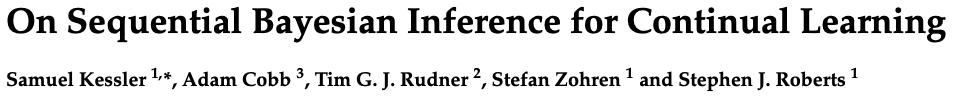
\includegraphics[width=\textwidth]{"images/title.png"}
        % \caption{February 2024}
	\end{figure}

    % \vspace{3em}
    % \centering
    % February 2024
\end{frame}

 %%%%%%%%%%%%%%%%%%%%%%%%%%%%%%%

\begin{frame}{Table of Contents}
    \tableofcontents
\end{frame}

%%%%%%%%%%%%%%%%%%%%%%%%%%%%%%%
\section{Continual Learning}
\begin{frame}{Continual Learning}
    \begin{column}{0.45\textwidth}
        In machine learning, most of the time we develop models assuming:
        \pause
        \begin{itemize}
            \item a fixed distribution over the data
            \pause
            \item a fixed objective function
        \end{itemize}
        \pause
        Continual learning (CL) considers the case where the data-distribution and/or objective function can change over time.
    \end{column}
    \begin{column}{0.05\textwidth}
    \hspace*{1em}
    \end{column}
    \begin{column}{0.5\textwidth}
        \pause
        \begin{figure}
    		% \centering
            \begin{center}
                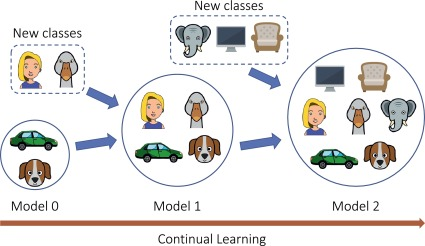
\includegraphics[width=0.8\textwidth]{"images/class_incremental_CL.jpg"}
                \caption{Class incremental CL \parencite{michieli_chapter_2022}.}
            \end{center}
    	\end{figure}
    \end{column}
\end{frame}

%%%%%%%%%%%%%%%%%%%%%%%%%%%%%%%
\begin{frame}{Continual Learning: Tasks}
\begin{itemize}
    \item We split a CL setting into a series of consecutive tasks $$\mathcal{T}_1,\mathcal{T}_2,\mathcal{T}_3,\ldots$$ where we believe each task has a fixed distribution over the data and a fixed objective function.

    \pause 
    \item i.e. task $\mathcal{T}_t$ is comprised of a dataset $\mathcal{D}_t = \{(x_i,y_i)\}_{i=1}^{N_t}$
    \pause
    \item The challenge is to learn sequentially on each task \textbf{without forgetting what was learnt in previous tasks}.
\end{itemize}
\end{frame}

%%%%%%%%%%%%%%%%%%%%%%%%%%%%%%%
\begin{frame}{Continual Learning: Cases}
    \cite{lesort_continual_2019} provide some good examples where CL is necessary:
    % \begin{column}{0.5\textwidth}
        \begin{itemize}[<+->]
            \item You want to update a trained model but no longer have access to the original training data.
            \item You want to train a model on a sequence of tasks but can't use the whole dataset at once (due to memory or computational constraints).
            \item You want an agent that learns multiple policies but you don't know when/how the learning objective changes.
            \item You want to learn from a continuous stream of data that changes through time (and perhaps you don't know when/how).
        \end{itemize}
    
\end{frame}

%%%%%%%%%%%%%%%%%%%%%%%%%%%%%%%
\begin{frame}{Continual Learning: Examples}

\begin{figure}
    \centering
    \begin{center}
        \hspace*{1cm}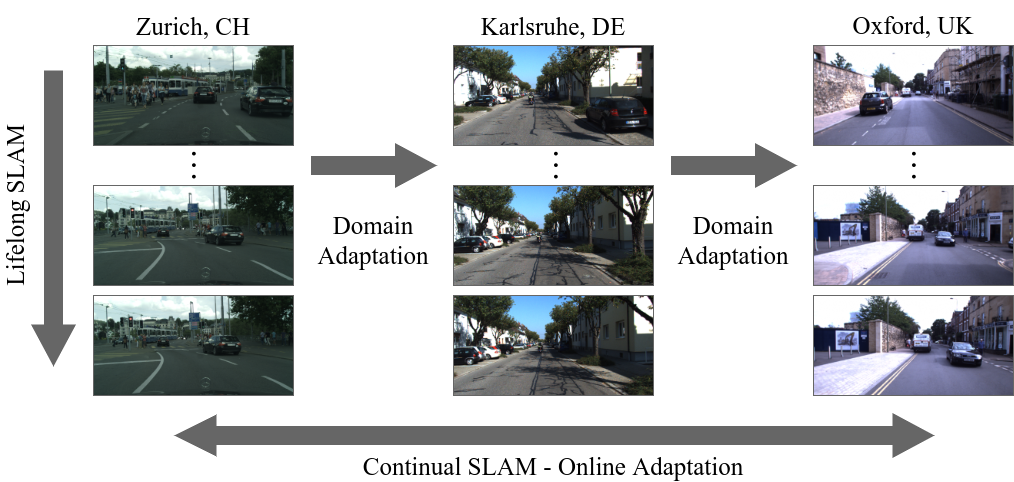
\includegraphics[width=0.8\textwidth]{"images/continual_slam.png"}
        \caption{Continual SLAM \parencite{vodisch_continual_2023}.}
    \end{center}
\end{figure}
    
\end{frame}

%%%%%%%%%%%%%%%%%%%%%%%%%%%%%%%
\begin{frame}{Continual Learning: Examples}

\begin{figure}
    \centering
    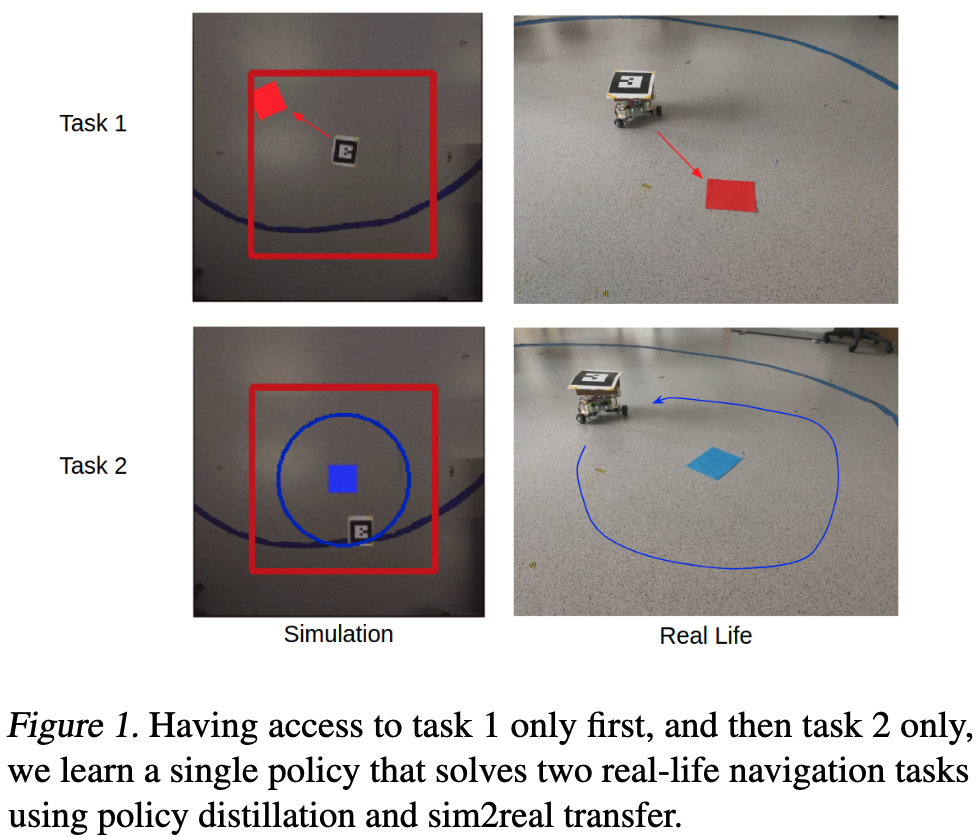
\includegraphics[width=0.4\textwidth]{"images/robot2task.png"}
        \caption{Sequential Objectives \parencite{traore_continual_2019}.}
\end{figure}
    
\end{frame}

%%%%%%%%%%%%%%%%%%%%%%%%%%%%%%%
\begin{frame}{Continual Learning: Examples}

\begin{figure}
    % \centering
    \begin{center}
        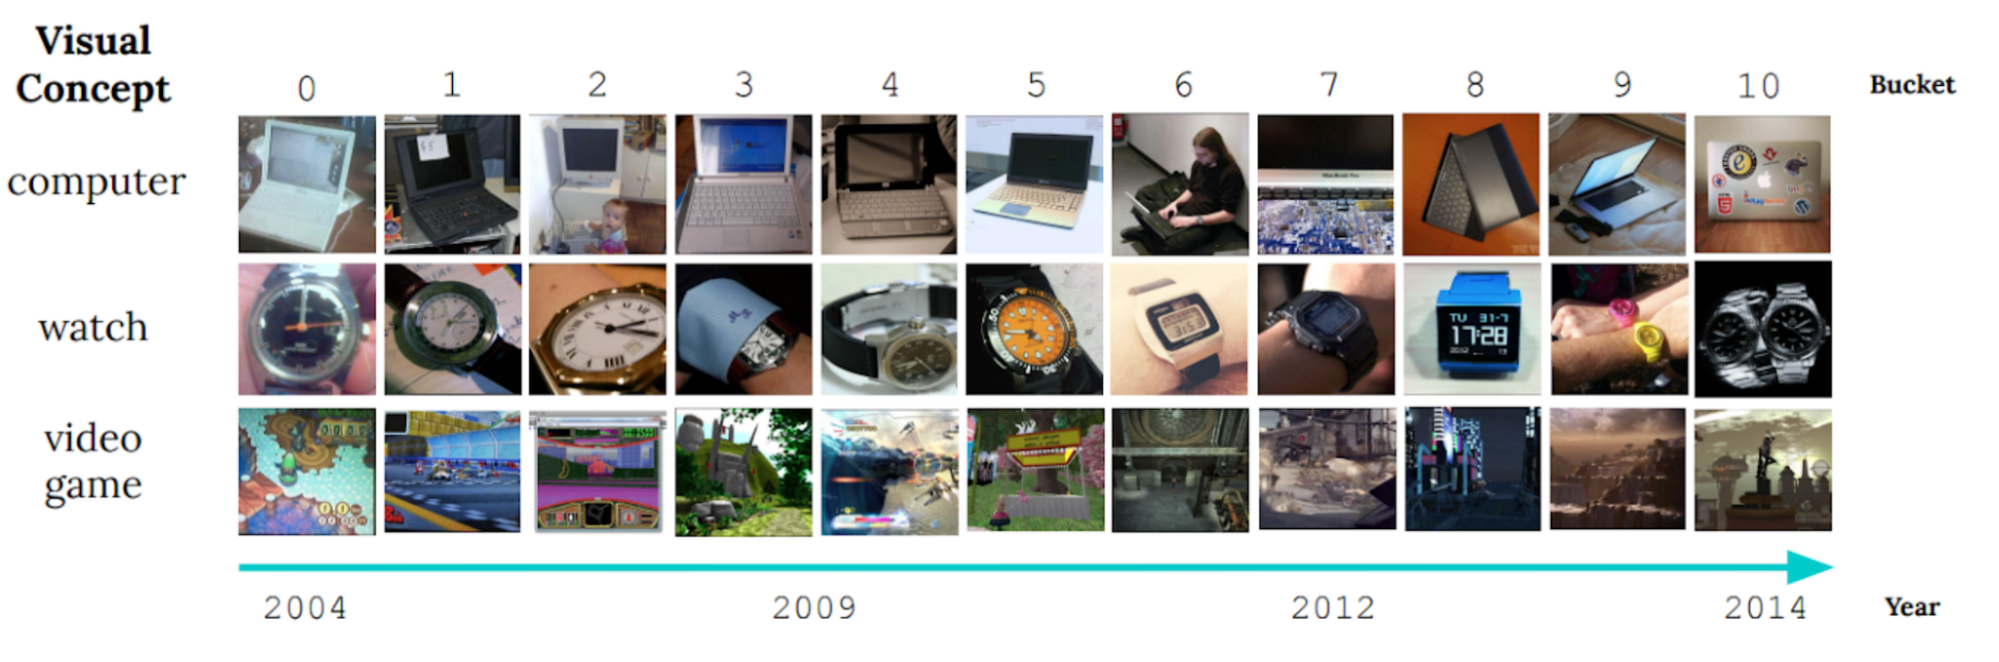
\includegraphics[width=\textwidth]{"images/concept_drift.png"}
        \caption{Conceptual Drift \parencite{jain_instance-conditional_2023}.}
    \end{center}
\end{figure}
    
    
\end{frame}



%%%%%%%%%%%%%%%%%%%%%%%%%%%%%%%
\begin{frame}{Continual Learning Settings}

 % different types of CL (incl. SH vs MH)
 \begin{itemize}[<+->]
     \item \textbf{Task-incremental}: The model is allowed to know which task the test data comes from (so output space is task-dependent).
     \item \textbf{Domain-incremental}: The model doesn't know which task the test data comes from, and each task uses an equivalent but separate output space.
    %  at each stage of training the output space is identical.
    %  (e.g. Split-MNIST might become odd/even prediction if output space is $\{0,1\}$.)
    % \begin{itemize}
    %      \item Sequential Bayesian inference with Bernoulli likelihood.
     % \end{itemize}     
     \item \textbf{Class-incremental}: The model doesn't know which task the test data comes from, and the output space is shared across tasks.
     % at each stage of training the true output space effectively grows.
     % (e.g. Split-MNIST output space for all tasks is $\{0,\ldots,9\}$.)
     % \begin{itemize}
     %     \item Sequential Bayesian inference with categorical likelihood.
     % \end{itemize}
 \end{itemize}

\end{frame}

%%%%%%%%%%%%%%%%%%%%%%%%%%%%%%%
\begin{frame}{Continual Learning: Split-MNIST}

MNIST but each task only contains training points from two classes.

\begin{figure}
    \centering
    % \begin{center}
        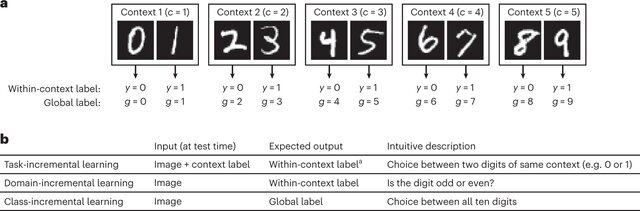
\includegraphics[width=0.8\textwidth]{"images/split_mnist.png"}
        \caption{Split MNIST \parencite{van_de_ven_three_2022}.}
    % \end{center}
\end{figure}
\end{frame}

%%%%%%%%%%%%%%%%%%%%%%%%%%%%%%%
\begin{frame}{Continual Learning Settings}

 % different types of CL (incl. SH vs MH)
 \begin{itemize}[<+->]
     \item \textbf{Single-headed}: Use the same model for all tasks.
     \item \textbf{Multi-headed}: Use a base model $f$ for all tasks, but train separate heads $g_t$ for each task and use some composition/combination of the heads at test time.
     \pause 
     \begin{itemize}
         \item (Or just pick the correct head if you know which task the test data comes from.)
     \end{itemize}
 \end{itemize}

\end{frame}

%%%%%%%%%%%%%%%%%%%%%%%%%%%%%%%
\section{Sequential Bayes}
\begin{frame}{Sequential Bayesian Inference} 
    % \cite{kessler_sequential_2023} suggest that sequential Bayesian inference \textit{should} be well suited for CL... \pause but in practice it usually isn't.
    % Task data arrives sequentially at timesteps $t=1,2,\ldots,T$.
    \vspace{1em}
    \begin{itemize}[<+->]
        \item At $t=1$ (for task $\mathcal{T}_1$) the posterior predictive for test point $x_1^* \in \mathcal{D}_1$:
        $$p(y_1^* | x_1^*, \mathcal{D}_1) = \int p(y_1^* | x_1^*, \theta)p(\theta | \mathcal{D}_1)d\theta$$
        % Note that this requires the posterior $p(\theta|\mathcal{D}_1)$.
        \item At $t=2$ (for task $\mathcal{T}_2$) the posterior predictive for test point $x_2^* \in \mathcal{D}_1 \cup \mathcal{D}_2$:
        $$p(y_2^* | x_2^*, \mathcal{D}_1, \mathcal{D}_2) = \int p(y_2^* | x_2^*, \theta)p(\theta | \mathcal{D}_1, \mathcal{D}_2)d\theta$$
        \item Each time step $T$ we receive $\mathcal{D}_T$ and update the posterior over $\theta$:
        $$p(\theta|\mathcal{D}_1,\ldots,\mathcal{D}_{T-1},\mathcal{D}_T) = \frac{p(\mathcal{D}_T | \theta)p(\theta|\mathcal{D}_1,\ldots,\mathcal{D}_{T-1})}{p(\mathcal{D}_T|\mathcal{D}_1,\ldots,\mathcal{D}_{T-1})}$$
    \end{itemize}

    

 %    \begin{figure}
	% 	\centering
	% 	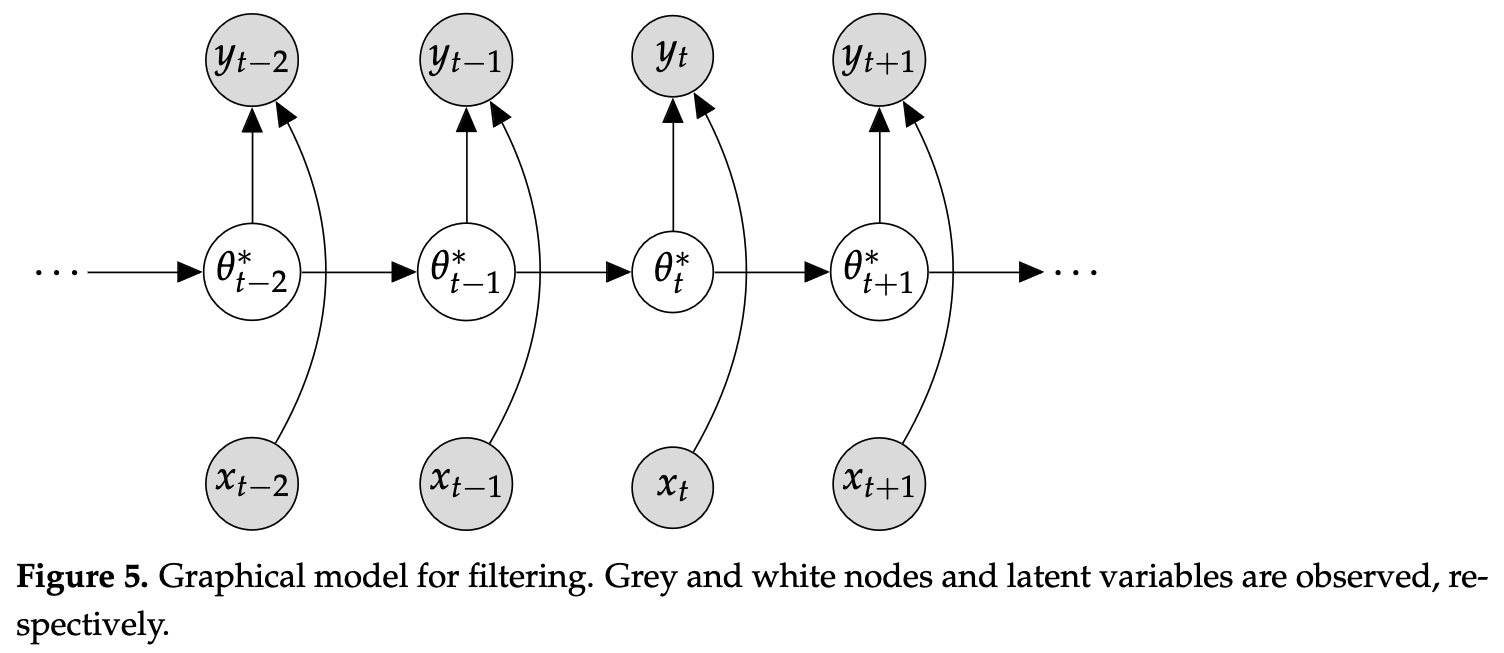
\includegraphics[width=\textwidth]{"images/Fig5_full.png"}
 %        % \caption{Credit: Johann Brehmer \parencite{brehmer_slides2022simulation_based_inference_rodem_sinergia_2022pdf_2022}.}
	% \end{figure}
\end{frame}

%%%%%%%%%%%%%%%%%%%%%%%%%%%%%%%
\begin{frame}{Sequential Bayesian Inference}
\begin{itemize}
    \item Each time step $T$ we receive $\mathcal{D}_T$ and update the posterior over $\theta$:
        $$p(\theta|\mathcal{D}_1,\ldots,\mathcal{D}_{T-1},\mathcal{D}_T) = \frac{p(\mathcal{D}_T | \theta)p(\theta|\mathcal{D}_1,\ldots,\mathcal{D}_{T-1})}{p(\mathcal{D}_T|\mathcal{D}_1,\ldots,\mathcal{D}_{T-1})}$$
    (assuming the datasets $\mathcal{D}_1,\ldots,\mathcal{D}_T$ are conditionally independent given $\theta$).
    \pause
    \begin{itemize}[<+->]
        \item $p(\mathcal{D}_T | \theta)$ doesn't require previous datasets.
        \item $p(\theta|\mathcal{D}_1,\ldots,\mathcal{D}_{T-1})$ is the posterior of time step $T-1$ and can be seen as the prior for time step $T$.
        \item $p(\mathcal{D}_T|\mathcal{D}_1,\ldots,\mathcal{D}_{T-1})$ is a constant we can ignore (sort of).
    \end{itemize}
\end{itemize}
    
\end{frame}

%%%%%%%%%%%%%%%%%%%%%%%%%%%%%%%
% \begin{frame}{Sequential Bayesian Inference}
% At $t=1$ the posterior is
% $$\log p(\theta | \mathcal{D}_1) = \log p(\mathcal{D}_1|\theta) + \log p(\theta) - \log p(\mathcal{D}_1)$$
% \pause
% At $t=2$ the posterior is 
% $$\log p(\theta | \mathcal{D}_1, \mathcal{D}_2) = \log p(\mathcal{D}_2|\theta) + \log p(\theta | \mathcal{D}_1) - \log p(\mathcal{D}_2 | \mathcal{D}_1)$$
% assuming conditional independence of $\mathcal{D}_1$ and $\mathcal{D}_2$ given $\theta$.
% \pause

% \begin{itemize}[<+->]
%     \item $\log p(\mathcal{D}_2|\theta)$ doesn't require previous datasets.
%     \item $\log p(\theta | \mathcal{D}_1)$ is the posterior of $t=1$ and can be seen as the prior for $t=2$.
%     \item $\log p(\mathcal{D}_2 | \mathcal{D}_1)$ is a constant we can ignore.
% \end{itemize}
    
% \end{frame}


%%%%%%%%%%%%%%%%%%%%%%%%%%%%%%%
\begin{frame}{This Paper's Thesis}
    \cite{kessler_sequential_2023}:
    \begin{itemize}[<+->]
        \item Sequential Bayesian inference \textit{should} be well suited for CL...
        \item But over \textbf{the weights of} a BNN, sequential Bayes isn't actually very good in practice.
        \begin{enumerate}[<+->]
            \item Even if a BNN is a well-specified/flexible-enough model for the posterior.
            \item Even if we are able to perform high-quality inference.
            \item In part due to class imbalance across tasks.
        \end{enumerate}
        \item However, if we do sequential Bayes on the model in some lower-dimension latent space, might we get better results?
    \end{itemize}

\end{frame}

%%%%%%%%%%%%%%%%%%%%%%%%%%%%%%%
\section{VCL}
\begin{frame}{Variational Continual Learning (VCL)}

% \begin{columns}
%     \begin{column}{0.6\textwidth}
        
%     \end{column}
    
%     \begin{column}{0.4\textwidth}
%         \begin{figure}
%             \centering
%             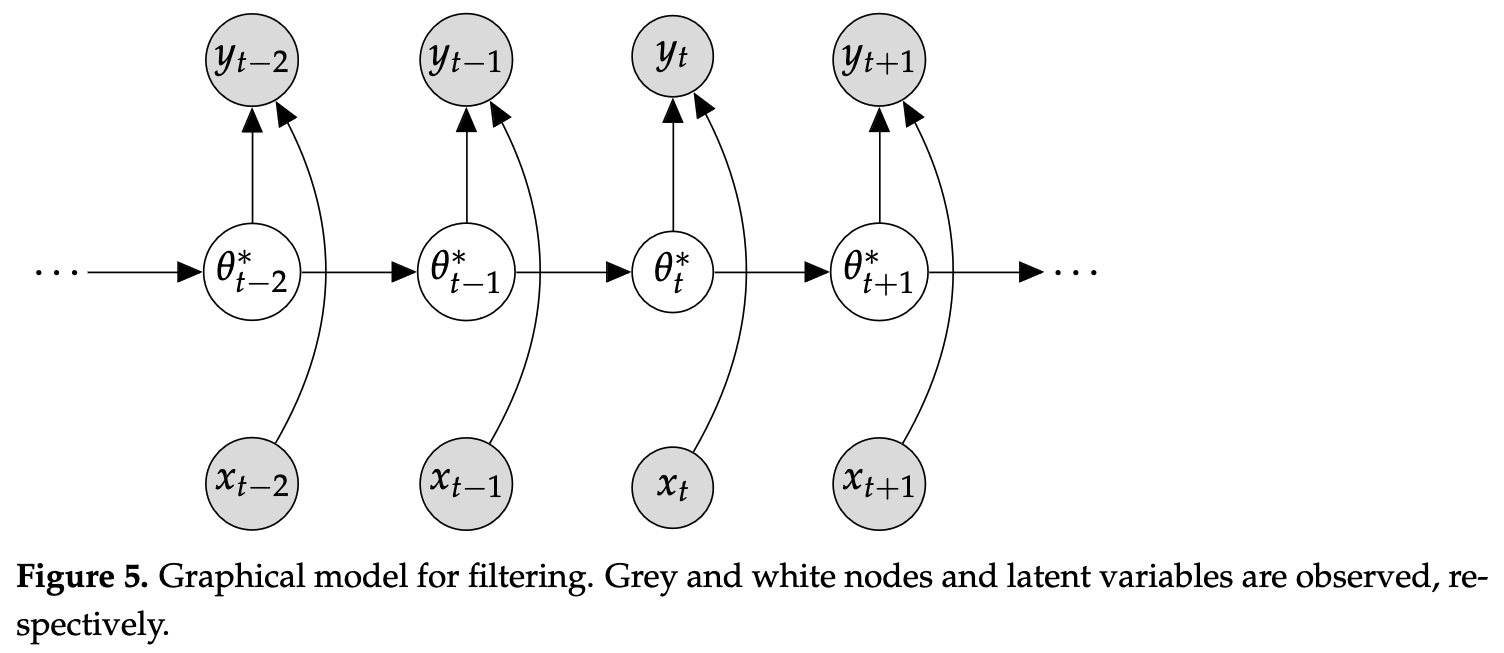
\includegraphics[height=0.62\textheight]{"images/Fig5_full.png"}
%             % \caption{\cite{cranmer_frontier_2020}}
%         \end{figure}
%     \end{column}
% \end{columns}

One generic solution: optimise an approximate posterior $q_t(\theta|\mathcal{D}_{1:t}) = \vcentcolon q_t(\theta)$ at each time step $t$ via \parencite{nguyen_variational_2018}:

\pause
$$\mathcal{L}(\theta | \mathcal{D}_t) = \mathbb{D}_{KL}[q_t(\theta) || q_{t-1}(\theta | \mathcal{D}_{1:t-1})] - \mathbb{E}_{q_t}[\log p(\mathcal{D}_t|\theta)].$$

\pause
Use single- and multi-headed versions (SH and MH respectively).

\end{frame}

%%%%%%%%%%%%%%%%%%%%%%%%%%%%%%%
\begin{frame}{VCL vs SGD (on a 2-layer BNN)}

\begin{figure}
    \centering
    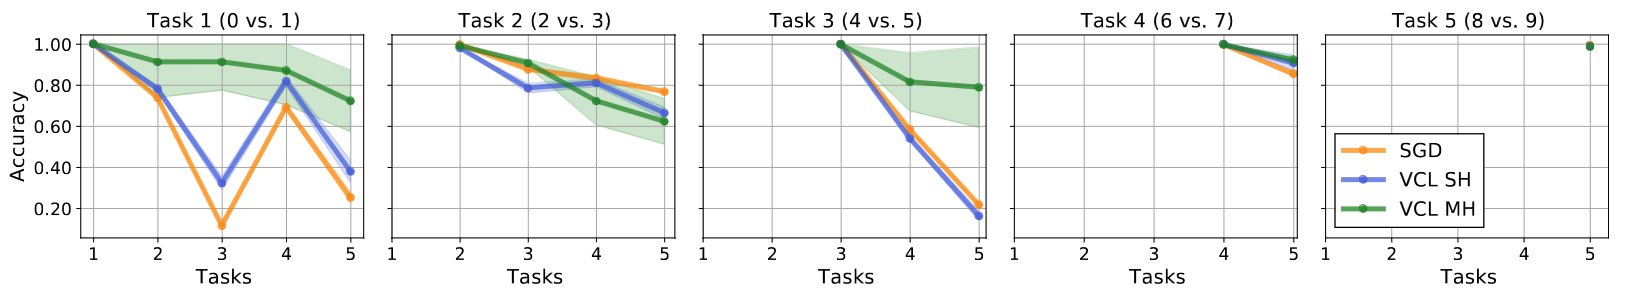
\includegraphics[width=\textwidth]{"images/Fig1_pic.png"}
    % \caption{\cite{cranmer_frontier_2020}}
\end{figure}

\pause
\begin{itemize}[<+->]
    \item VCL-MH is kind of cheating (and shouldn't really be necessary)
    \item What's worrying is that VCL-SH is pretty much the same as SGD
\end{itemize}

\pause
Hypothesis: the failure is due to imperfect approximate inference of the posterior(s).

\end{frame}

%%%%%%%%%%%%%%%%%%%%%%%%%%%%%%%
\section{HMC}
\begin{frame}{HMC}
\begin{column}{0.4\textwidth}
    \begin{figure}
		\centering
		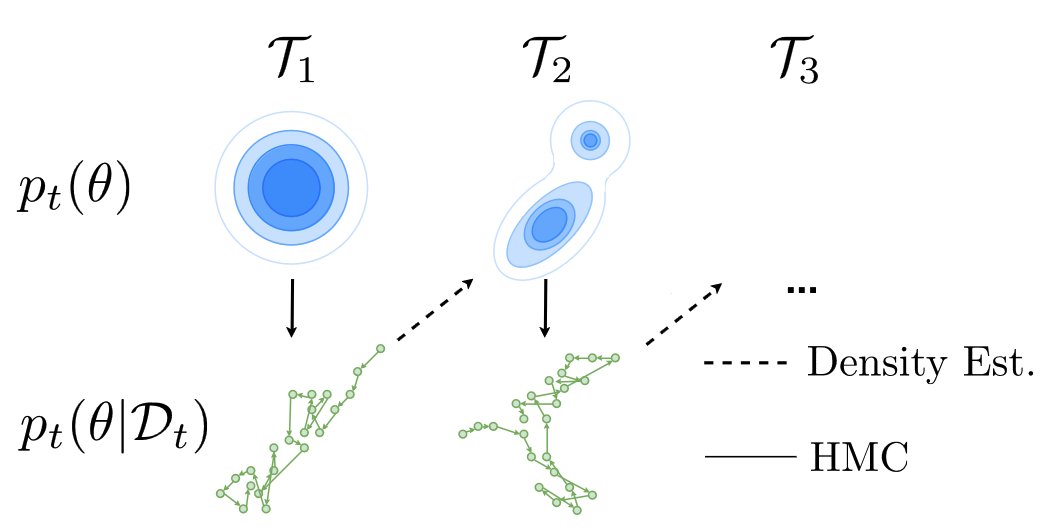
\includegraphics[width=\textwidth]{"images/Fig2_pic.png"}
	\end{figure}
\end{column}
\begin{column}{0.6\textwidth}
    Let's try the gold standard for inference: HMC
    \begin{itemize}[<+->]
        \item Start with prior
        \item Get posterior samples from task 1 via HMC
        \item Turn those samples into a GMM approx. posterior via by density estimation
        \item Repeat with this approx posterior as the new prior for task 2, \&c.
    \end{itemize}
\end{column}

\end{frame}

%%%%%%%%%%%%%%%%%%%%%%%%%%%%%%%
\begin{frame}{Trying HMC for better inference}
    \begin{figure}
		\centering
		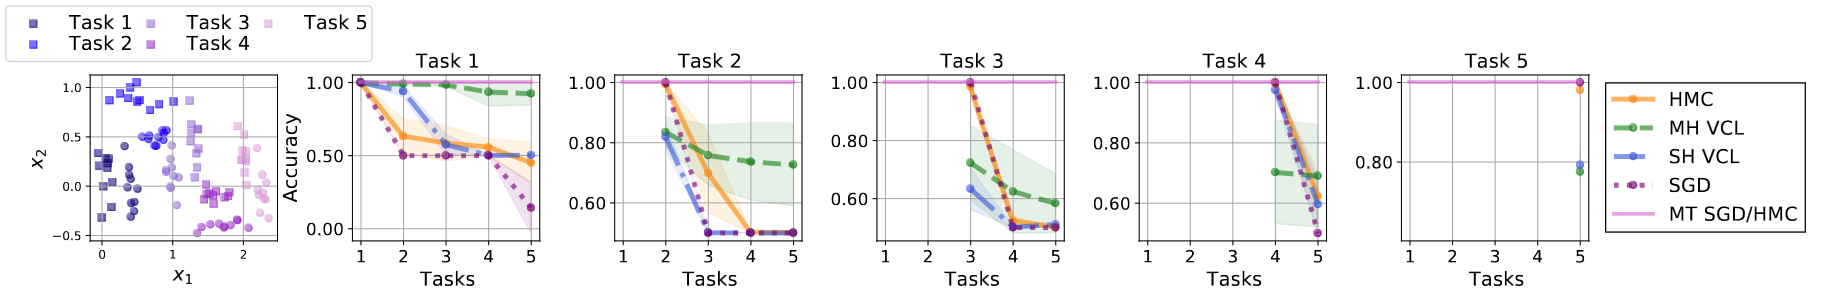
\includegraphics[width=\textwidth]{"images/Fig3_pic.png"}
	\end{figure}
    \vspace{-1em}
    \begin{figure}
		\centering
		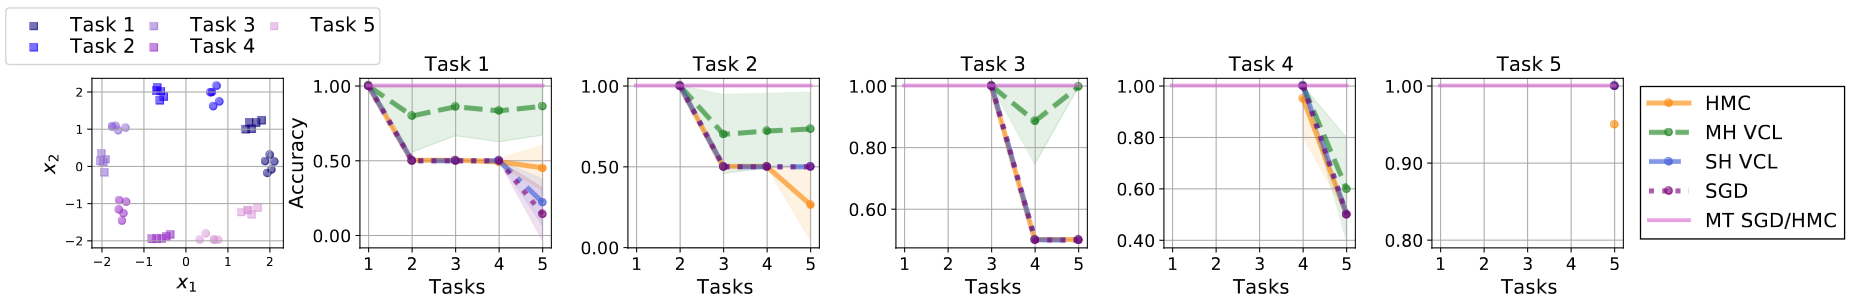
\includegraphics[width=\textwidth]{"images/FigA1_pic.png"}
	\end{figure}
 
    % % Even more worrying than (SH) VCL's poor performance: 
    % HMC is only marginally better than SGD
    % % (when HMC is usually a silver bullet for Bayesian inference tasks)
    
    % See pink line: if trained on all tasks at once, both HMC and SGD manage perfectly, so model is flexible enough to learn full posterior.

    \begin{itemize}
        \item HMC is only marginally better than SGD.
        % \item See pink line: if trained on all tasks at once, both HMC and SGD manage perfectly, so model is flexible enough to learn full posterior.
    \end{itemize}
 
\end{frame}

%%%%%%%%%%%%%%%%%%%%%%%%%%%%%%%
\section{Why doesn't it work?}
\begin{frame}{Why doesn't it work?}

Two potential reasons:
\begin{enumerate}
    \item Model misspecification
    \item Imperfect inference
\end{enumerate}

\end{frame}

%%%%%%%%%%%%%%%%%%%%%%%%%%%%%%%
\begin{frame}{Model Misspecification}
\begin{itemize}
    \item Consider the simple model where $\theta_1, \theta_2, \ldots, \theta_t \sim p$ and observations arrive online (with known $\sigma$):
    $$p(y_t | \theta_t) = \mathcal{N}(y_t; \theta_t, \sigma^2)$$
    \pause
    \item We want to infer the filtering distribution $p(\theta_t | y_1,\ldots,y_t)$.
    \pause
    \item We can perform exact sequential Bayesian inference via closed-form updates:
    $$\hat{\theta}_t = \hat{\sigma}_t^2 \left( \frac{y_t}{\sigma^2} + \frac{\hat{\theta}_{t-1}}{\hat{\sigma}_{t-1}^2}  \right) = \hat{\sigma}_t^2 \left( \sum_{i=1}^t \frac{y_i}{\sigma^2} + \frac{\hat{\theta}_{0}}{\hat{\sigma}_{0}^2}  \right), \;\; \frac{1}{\hat{\sigma}_t^2} = \frac{1}{\sigma^2} + \frac{1}{\hat{\sigma_{t-1}^2}}$$
    Given some prior $p(\hat{\theta}_0) = \mathcal{N}(\theta_0; 0, \sigma_0^2)$.
\end{itemize}

\end{frame}

%%%%%%%%%%%%%%%%%%%%%%%%%%%%%%%
\begin{frame}{Model Misspecification}
\begin{itemize}[<+->]

    \item Try to model changepoint detection where data moves from a $\mathcal{N}(-1,\sigma^2)$ distribution to $\mathcal{N}(1,\sigma^2)$ after some number of time steps ($\theta$ moves from -1 to 1).
    \pause
    \begin{figure}
        \centering
        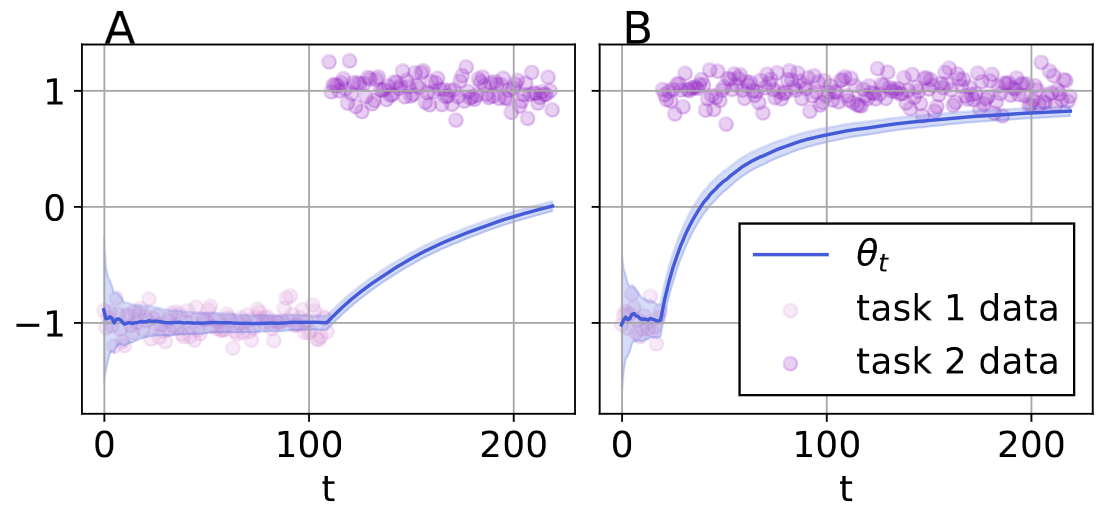
\includegraphics[width=0.4\textwidth]{"images/Fig4_pic.png"}
    \end{figure}
    
    \item A linear model doesn't work when subsequent tasks have different modes (kind of obvious). It will track the global mean.
    \item ``\textit{Despite performing exact inference, a misspecified model can forget}''
\end{itemize}

\end{frame}

%%%%%%%%%%%%%%%%%%%%%%%%%%%%%%%
\begin{frame}{Model Misspecification}

    \begin{figure}
		\centering
		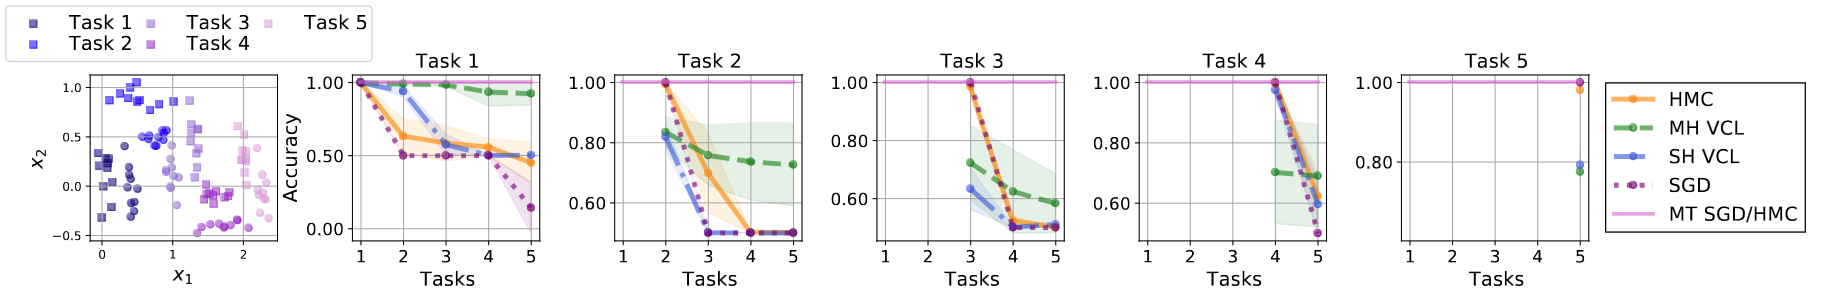
\includegraphics[width=\textwidth]{"images/Fig3_pic.png"}
	\end{figure}

 %    \begin{figure}
	% 	\centering
	% 	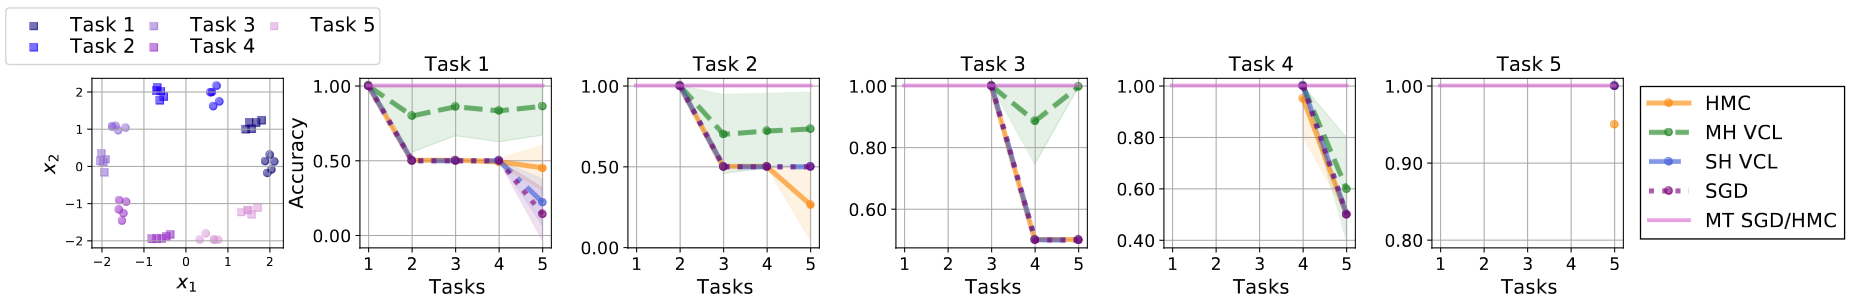
\includegraphics[width=\textwidth]{"images/FigA1_pic.png"}
	% \end{figure}

\begin{itemize}[<+->]
    \item Note that in the previous experiment we don't think that the BNN is misspecified: when trained on all tasks at once the BNN is able to get 100\% accuracy (pink line).
    \item So it must be a problem with the way sequential Bayesian inference works on a BNN.
\end{itemize}

\end{frame}

%%%%%%%%%%%%%%%%%%%%%%%%%%%%%%%
\begin{frame}{Imbalanced Task Data}
 %    \begin{figure}
	% 	\centering
	% 	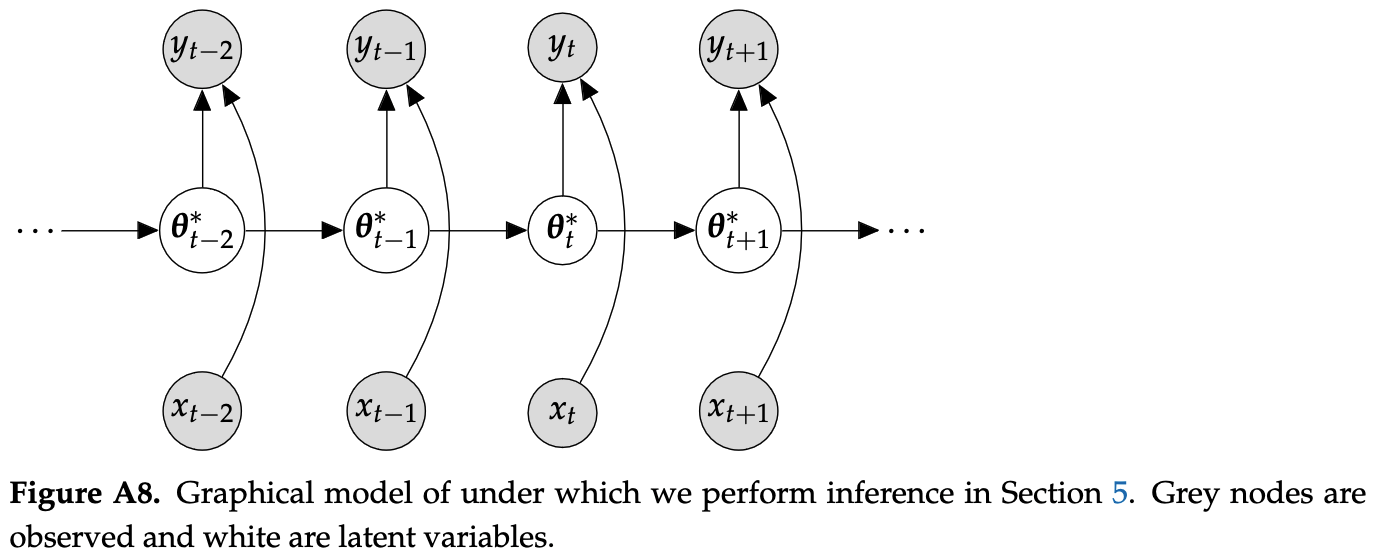
\includegraphics[width=\textwidth]{"images/FigA8_full.png"}
	% \end{figure}
    

    % Looking at BNN maths (via Fig. 5 or Fig A8) , we see that, under some (reasonable?) assumptions, if there is imbalanced task data the posterior mean will move towards that of the more data-heavy task. (again, sort of obvious?/expected?)

    %  (the above is when we try to optimize $\theta$ at each time point hence $\theta_t^*$).

    % Therefore, we shouldn't do inference directly on the weights of the BNN.
    \begin{itemize}[<+->]
        \item The authors analyse a simplified model of sequential Bayes on a BNN.
        % \item They argue that, just like in the previous experiment, uneven amounts of data per task can also affect the posterior obtained as time goes on.
        \begin{figure}
    		\centering
    		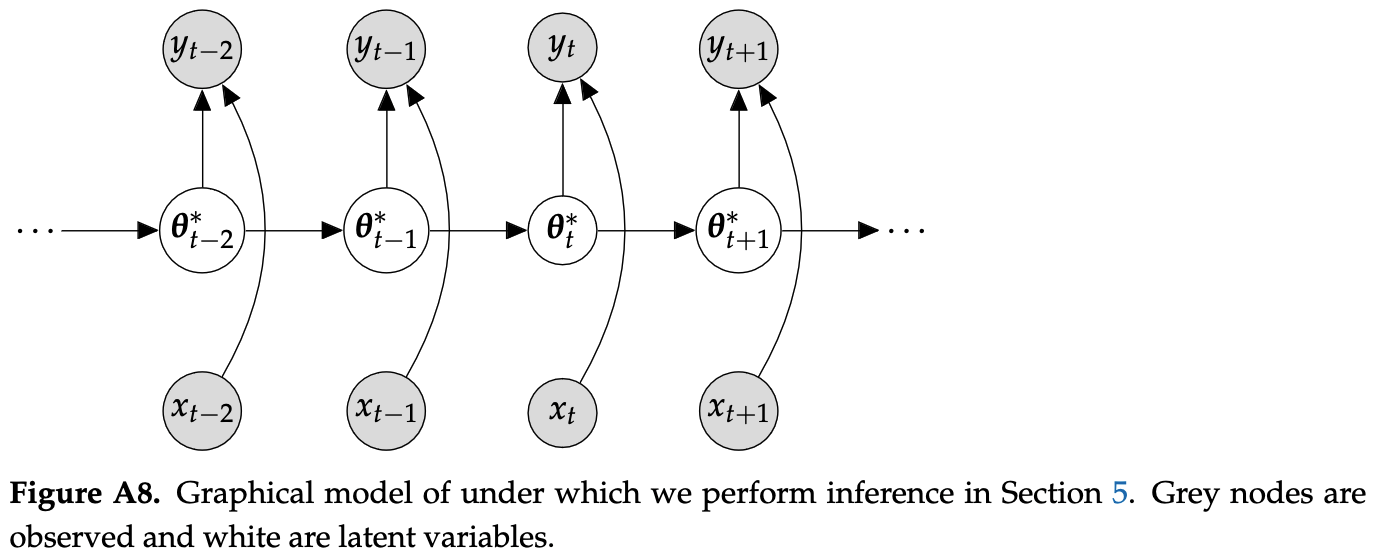
\includegraphics[width=0.8\textwidth]{"images/FigA8_full.png"}
    	\end{figure}
        % \item ``\textit{the posterior mean depends linearly on the prior and a data-dependent term and so will behave similarly to our previous example}''.
        % \pause
        % \item This is a problem because (task-incremental) CL algorithms almost always require the use of \textit{core sets} of data from previous tasks that are sprinkled into subsequent tasks to prevent catastrophic forgetting.
    \end{itemize}

\end{frame}

%%%%%%%%%%%%%%%%%%%%%%%%%%%%%%%
\begin{frame}{Imbalanced Task Data}
 %    \begin{figure}
	% 	\centering
	% 	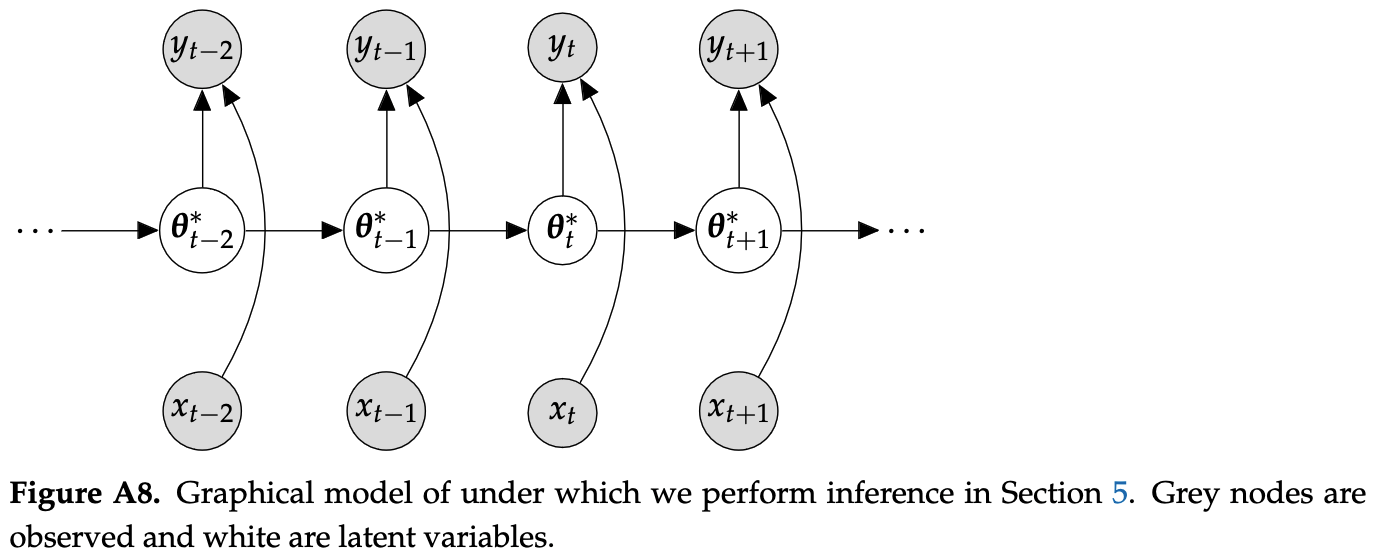
\includegraphics[width=\textwidth]{"images/FigA8_full.png"}
	% \end{figure}
    

    % Looking at BNN maths (via Fig. 5 or Fig A8) , we see that, under some (reasonable?) assumptions, if there is imbalanced task data the posterior mean will move towards that of the more data-heavy task. (again, sort of obvious?/expected?)

    %  (the above is when we try to optimize $\theta$ at each time point hence $\theta_t^*$).

    % Therefore, we shouldn't do inference directly on the weights of the BNN.
    \vspace{-1em}
    \begin{itemize}[<+->]
        % \item The authors analyse a simplified model of sequential Bayes on a BNN.
        \item They argue that, just like in the previous experiment, uneven amounts of data per task can also affect the posterior obtained as time goes on.
        \begin{figure}
    		\centering
    		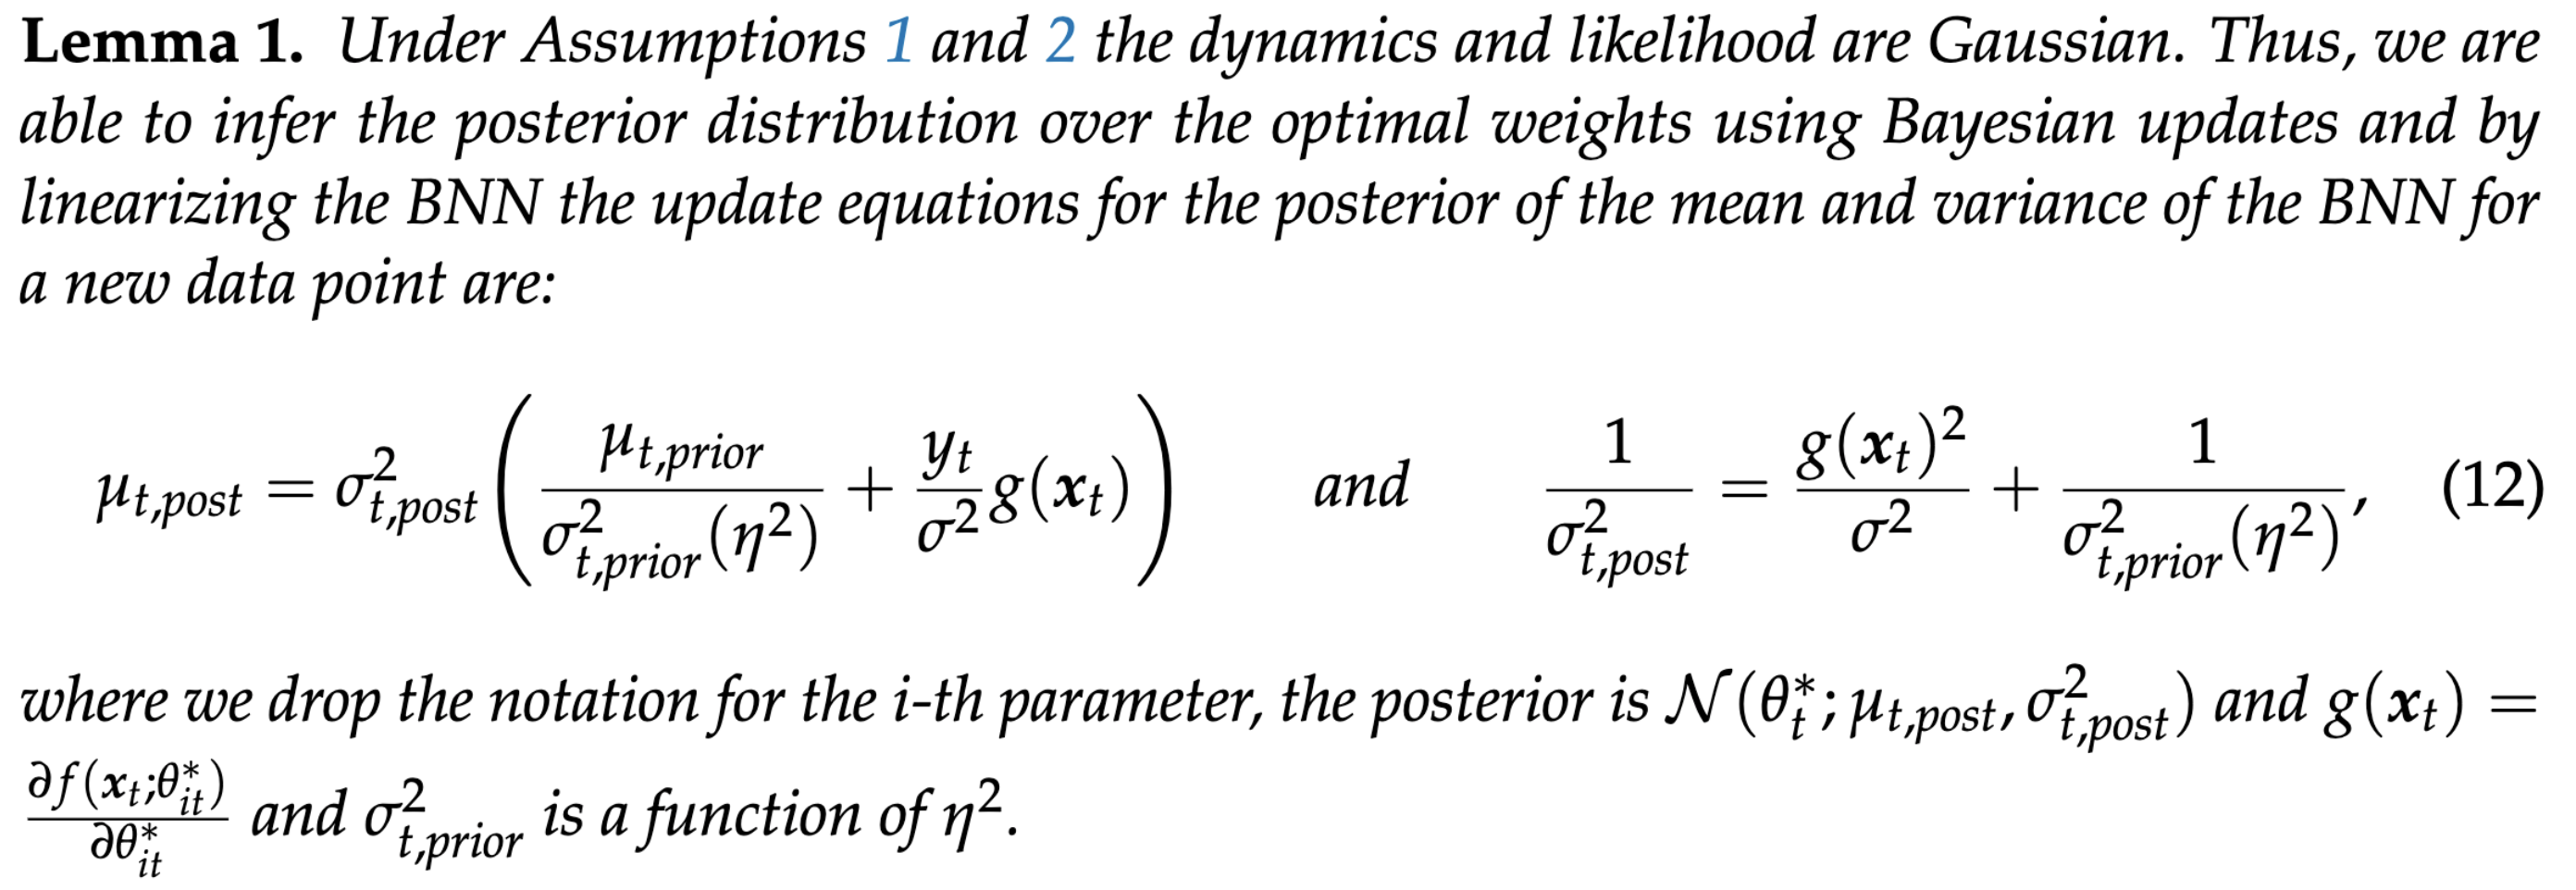
\includegraphics[width=0.7\textwidth]{"images/lemma1.png"}
    	\end{figure}
        % \pause
        % \item This is a problem because (task-incremental) CL algorithms almost always require the use of \textit{core sets} of data from previous tasks that are sprinkled into subsequent tasks to prevent catastrophic forgetting.
    \end{itemize}

\end{frame}

%%%%%%%%%%%%%%%%%%%%%%%%%%%%%%%
\begin{frame}{Imbalanced Task Data}
 %    \begin{figure}
	% 	\centering
	% 	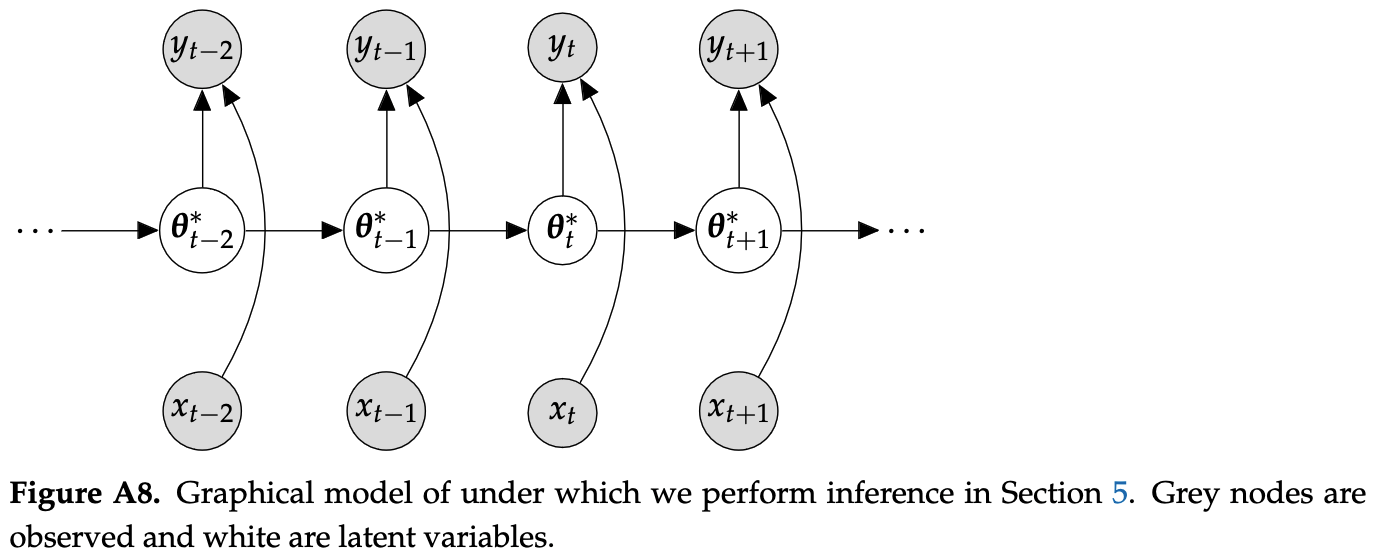
\includegraphics[width=\textwidth]{"images/FigA8_full.png"}
	% \end{figure}
    

    % Looking at BNN maths (via Fig. 5 or Fig A8) , we see that, under some (reasonable?) assumptions, if there is imbalanced task data the posterior mean will move towards that of the more data-heavy task. (again, sort of obvious?/expected?)

    %  (the above is when we try to optimize $\theta$ at each time point hence $\theta_t^*$).

    % Therefore, we shouldn't do inference directly on the weights of the BNN.
    \begin{itemize}
        % \item The authors analyse a simplified model of sequential Bayes on a BNN.
        \item They argue that, just like in the previous experiment, uneven amounts of data per task can also affect the posterior obtained as time goes on.
        \begin{figure}
    		\centering
    		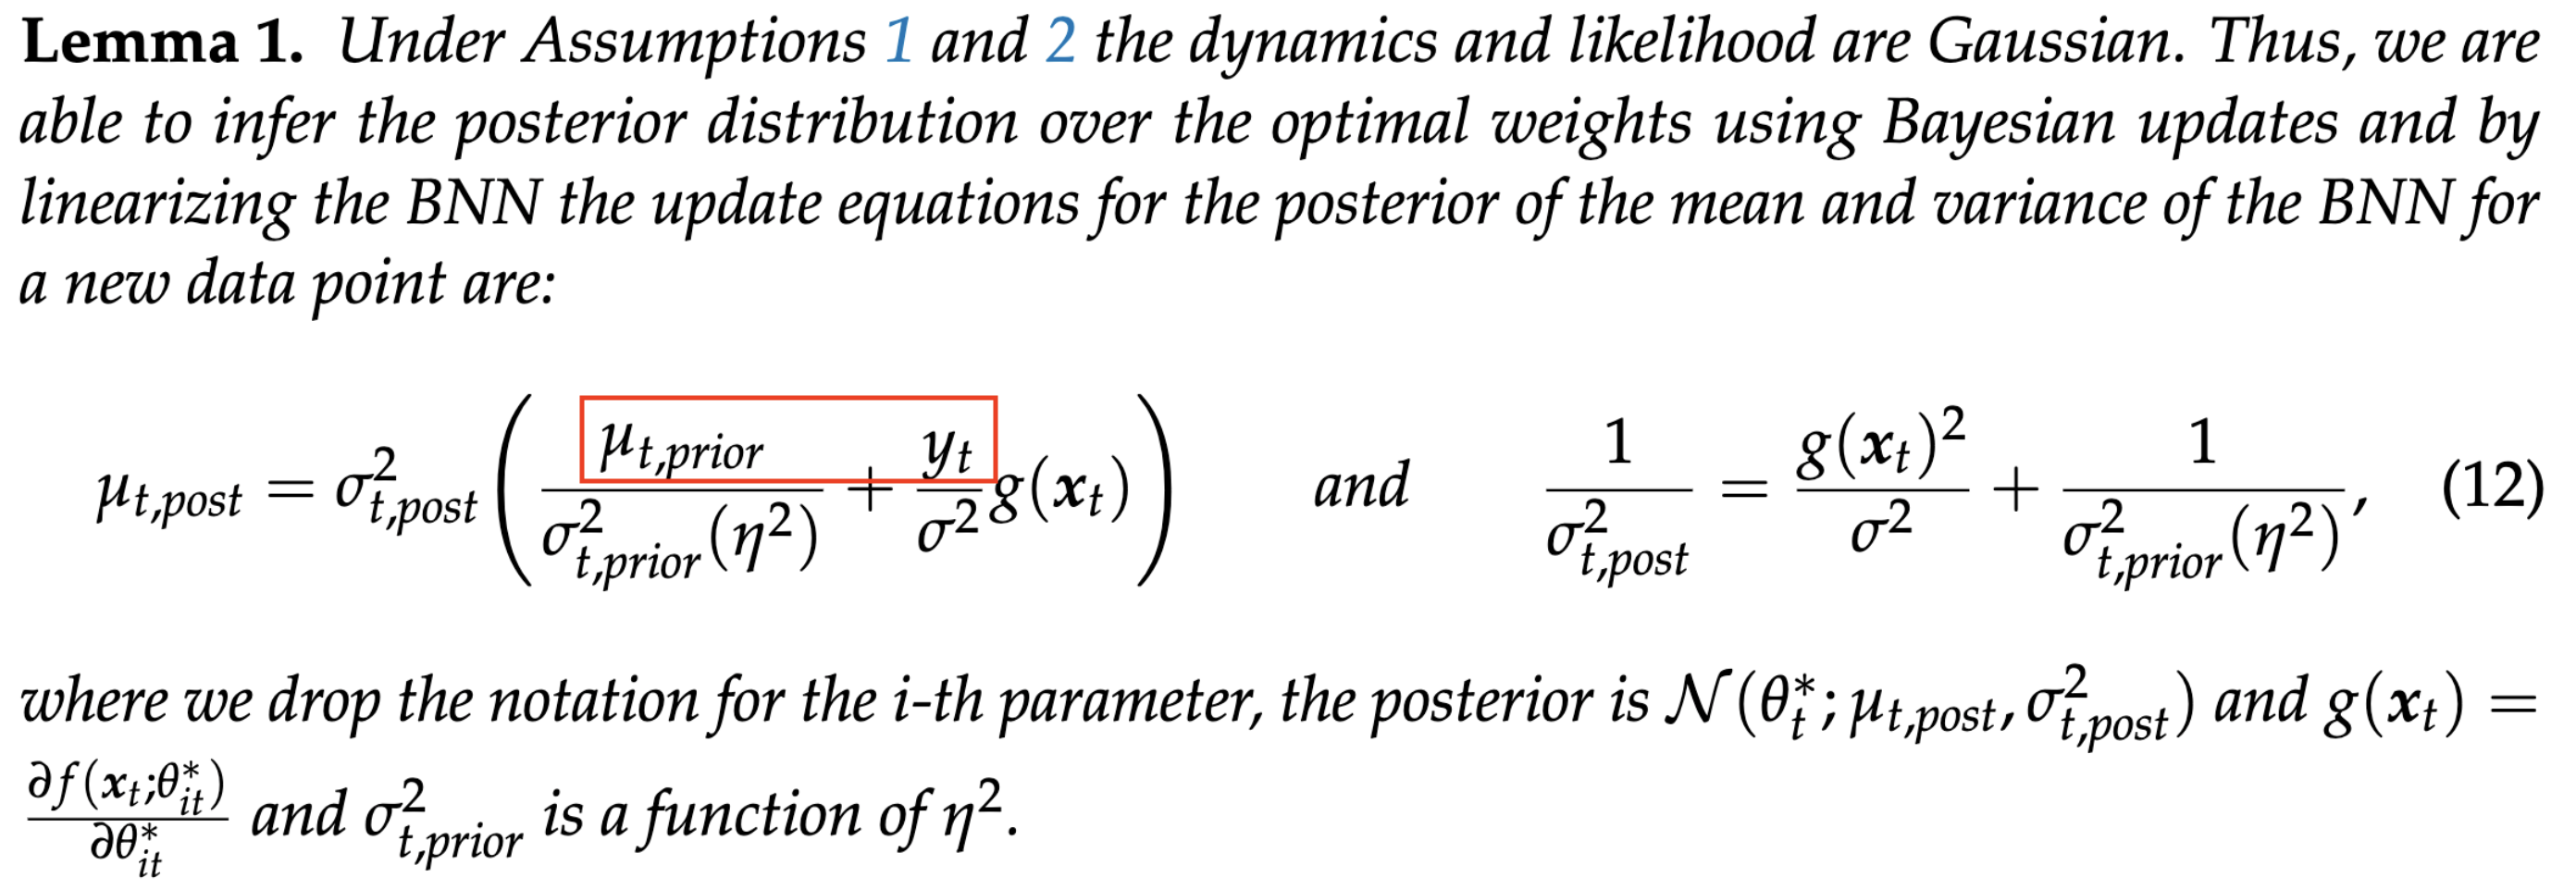
\includegraphics[width=0.7\textwidth]{"images/lemma1_annotated.png"}
    	\end{figure}
        \pause
        \item ``\textit{the posterior mean depends linearly on the prior and a data-dependent term and so will behave similarly to our previous example}''.
        % \pause
        % \item This is a problem because (task-incremental) CL algorithms almost always require the use of \textit{core sets} of data from previous tasks that are sprinkled into subsequent tasks to prevent catastrophic forgetting.
    \end{itemize}

\end{frame}

%%%%%%%%%%%%%%%%%%%%%%%%%%%%%%%
\begin{frame}{Imbalanced Task Data}
     \begin{itemize}[<+->]
        \item This is a problem for two main reasons:
        \begin{enumerate}
            \item In most online settings we might not know how long each task lasts for, i.e. how much data to expect per task.
            \item (Task-incremental) CL algorithms almost always require the use of \textit{core sets} of data from previous tasks.
            % \pause 
            \begin{itemize}
                \item These saved previous datapoints are sprinkled into subsequent tasks to prevent catastrophic forgetting.
            \end{itemize}
        \end{enumerate} 
    \end{itemize}

\end{frame}

%%%%%%%%%%%%%%%%%%%%%%%%%%%%%%%
\section{ProtoCL}
\begin{frame}{Prototypical Bayesian Continual Learning}
\begin{itemize}[<+->]
    \item \alert{Problem}: performing sequential Bayesian inference over BNN weights is probably a bad idea.
    \item \alert{Solution}: instead, do it over latent variables in an embedding space (where the embeddings come from a regular NN).
\end{itemize}
    
\end{frame}

%%%%%%%%%%%%%%%%%%%%%%%%%%%%%%%
\begin{frame}{ProtoCL Model}
\begin{columns}
    \begin{column}{0.4\textwidth}
        \begin{figure}
		\centering
		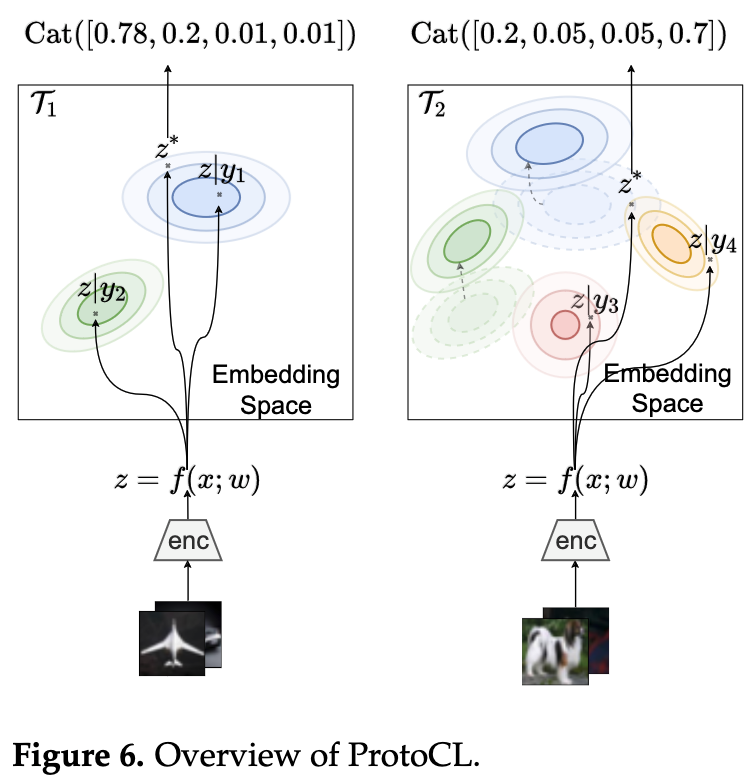
\includegraphics[width=0.8\textwidth]{"images/Fig6_full.png"}
	\end{figure}
    \end{column} 
    \begin{column}{0.6\textwidth}
        \begin{itemize}[<+->]
            \item Use regular NN to embed data points $z = f(x; w)$ with parameters $w$.
            \item Also keep track of Gaussian `prototype' distributions per class $y$ in the embedding space at time $t$.
            $$\bar{z}_{yt} \sim \mathcal{N}(\mu_{yt}, \Lambda_{yt}^{-1})$$
            
            \item We'll then use MAP estimates to assign class (based on which class prototype the embedding $z$ is closest to).
        \end{itemize}
    \end{column}
\end{columns}
\end{frame}

%%%%%%%%%%%%%%%%%%%%%%%%%%%%%%%
\begin{frame}{ProtoCL Model}
\begin{columns}
    \begin{column}{0.4\textwidth}
        \begin{figure}
		\centering
		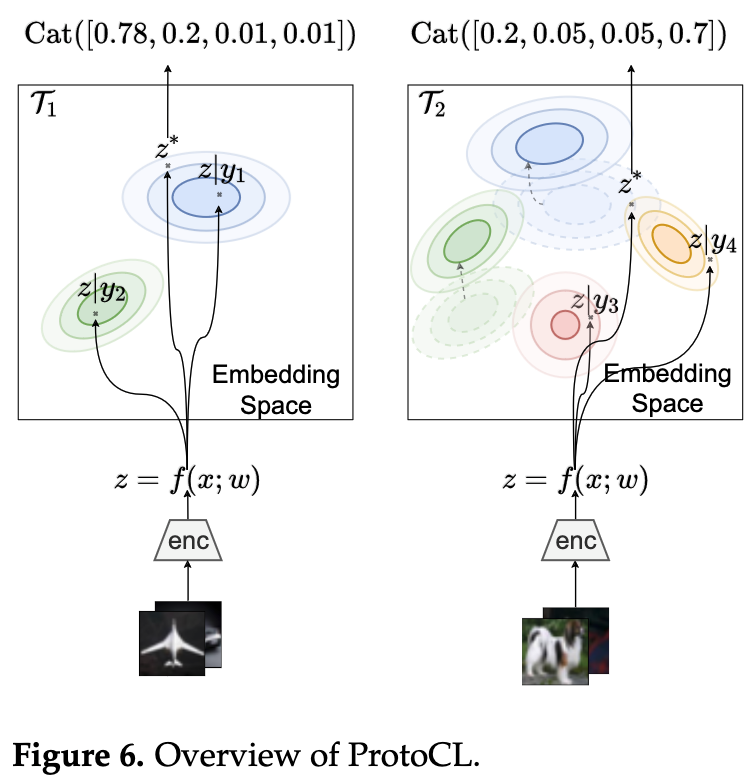
\includegraphics[width=0.8\textwidth]{"images/Fig6_full.png"}
	\end{figure}
    \end{column} 
    \begin{column}{0.6\textwidth}
        \begin{itemize}[<+->]
            \item For data point $i$ of task $t$, model $x_{i,t}$'s class $y_{i,t}$ via a categorical distribution with a Dirichlet prior:
            $$y_{i,t} \sim \mathrm{Cat}(p_{1:J}), \;\; p_{1:J} \sim \mathrm{Dir}(\alpha_t)$$
            \item Given a class $y_{i,t}$ we assume the embedding $z_{it}$ is distributed normally around the class' prototype $\bar{z}_{yt}$.
            $$z_{it} | y_{i,t} \sim \mathcal{N}(\bar{z}_{yt}, \Sigma_\epsilon), \;\; \bar{z}_{yt} \sim \mathcal{N}(\mu_{yt}, \Lambda_{yt}^{-1})$$
            % \item The posterior distribution over class probabilities $\{p_j\}_{j=1}^J$ and class embeddings $\{\bar{z}_{y_j}\}_{j=1}^J$ is denoted by $p(\theta)$ with parameters $\eta_t = \{\alpha_t, \mu_{1:J}, \Lambda_{1:J, t}^{-1}\}$
            
        \end{itemize}
    \end{column}
\end{columns}
\end{frame}


%%%%%%%%%%%%%%%%%%%%%%%%%%%%%%%
\begin{frame}{ProtoCL Model}
\begin{columns}
    \begin{column}{0.4\textwidth}
        \begin{figure}
		\centering
		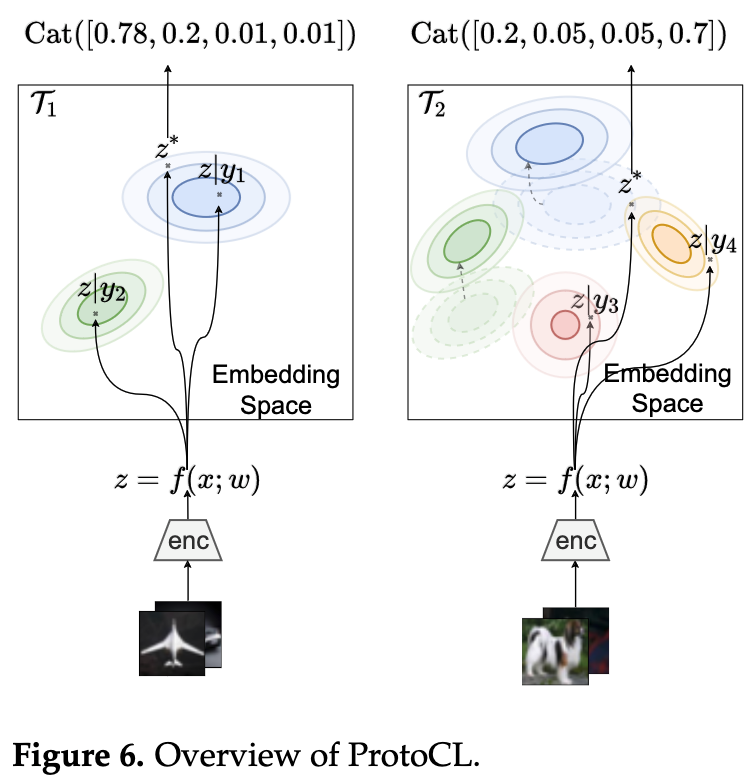
\includegraphics[width=0.8\textwidth]{"images/Fig6_full.png"}
	\end{figure}
    \end{column} 
    \begin{column}{0.6\textwidth}
        \begin{itemize}[<+->]
            \item The posterior distribution over 
            \begin{itemize}
                \item class probabilities $\{p_j\}_{j=1}^J$ and 
                \item class embeddings $\{\bar{z}_{y_j}\}_{j=1}^J$ (prototypes)
            \end{itemize} \pause is denoted by $p(\theta)$ with parameters $$\eta_t = \{\alpha_t, \mu_{1:J, t}, \Lambda_{1:J, t}^{-1}\}$$
            
        \end{itemize}
    \end{column}
\end{columns}
\end{frame}


%%%%%%%%%%%%%%%%%%%%%%%%%%%%%%%
\begin{frame}{ProtoCL Updates}
    $$\alpha_{t+1,j} = \alpha_{t,j} + \sum_{i=1}^{N_t}\mathbb{I}(y_t^i = j),$$
    where $N_t$ is the number of points seen during the update at timestep $t$.
    
    % \pause
    
    % \begin{align}
    % \nonumber
    %     \Lambda_{y_{t+1}} &= \Lambda_{y_t} + N_y \Lambda_\epsilon^{-1} \\
    % \nonumber
    %     \Lambda_{y_{t+1}}\mu_{y_{t+1}} &= \Lambda_{y_t}\mu_{y_t} + N_y \Lambda_\epsilon^{-1}\bar{z}_{y_t},  \; \forall y_t \in C_t
    % \end{align}
    % where $N_y$ is the number of samples of class $y$ and $\bar{z}_{y_t} = (1/N_y)\sum_{i=1}^N_y z_{yi}$.
\end{frame}

%%%%%%%%%%%%%%%%%%%%%%%%%%%%%%%
\begin{frame}{ProtoCL Update}

    (Update of $\alpha_t$ as tasks progress in Split MNIST.)
    
    \begin{figure}
		\centering
		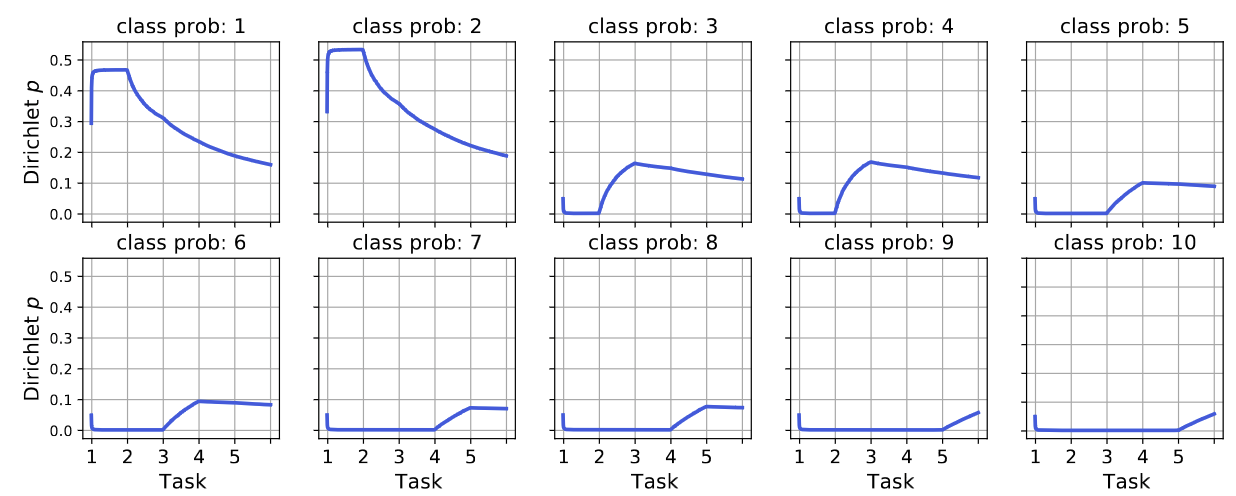
\includegraphics[width=0.9\textwidth]{"images/FigA7_pic.png"}
	\end{figure}
\end{frame}

%%%%%%%%%%%%%%%%%%%%%%%%%%%%%%%
\begin{frame}{ProtoCL Updates}
    $$\alpha_{t+1,j} = \alpha_{t,j} + \sum_{i=1}^{N_t}\mathbb{I}(y_t^i = j),$$
    where $N_t$ is the number of points seen during the update at timestep $t$.

    \pause 
    
    \begin{align}
    \nonumber
        \Lambda_{y_{t+1}} &= \Lambda_{y_t} + N_y \Lambda_\epsilon^{-1} \\
    \nonumber
        \mu_{y_{t+1}} &= \Lambda_{y_{t+1}}^{-1}(\Lambda_{y_t}\mu_{y_t} + N_y \Lambda_\epsilon^{-1}\bar{z}_{y_t}),  \; \forall y_t \in C_t
    \end{align}
    where $N_y$ is the number of samples of class $y$ and $\bar{z}_{y_t} = (1/N_y)\sum_{i=1}^{N_y} z_{yi}$.
\end{frame}

%%%%%%%%%%%%%%%%%%%%%%%%%%%%%%%
\begin{frame}{ProtoCL Objective}
    \begin{itemize}[<+->]
        \item Posterior predictive distribution of the embeddings $z$ and class labels $y$
    % $$p(z,y) = \int p(z,y | \theta_t;\eta_t)p(\theta_t;\eta_t)d\theta_t = p(y)\prod_{i=1}^{N_t} \mathcal{N}(z_{it} | y_{it}; \mu_{y_t, t}, \Sigma_\epsilon + \Lambda_{y_t, t}^{-1})$$
    $$p(z,y) = p(y)\prod_{i=1}^{N_t} \mathcal{N}(z_{it} | y_{it}; \mu_{y_t, t}, \Sigma_\epsilon + \Lambda_{y_t, t}^{-1})$$
    where $p(y) = \alpha_y / \sum_{j=1}^J \alpha_j$

        \item Optimize this objective with gradient-based optimization to learn embedding $z=f(x;w)$.
    \end{itemize}
\end{frame}

% %%%%%%%%%%%%%%%%%%%%%%%%%%%%%%%
% \begin{frame}{ProtoCL Predictions}
%     For a test point $x^*$ just choose the max (log-)posterior predictive:
%     $$p(y^* = j | x^*, x_{1:t}, y_{1:t}) = p(y^* = j| z^*, \theta_t) = \frac{p(y^* = j, z^* | \theta_t)}{\sum_i p(y^* = i, z^* | \theta_t)}$$
    
% \end{frame}


%%%%%%%%%%%%%%%%%%%%%%%%%%%%%%%
\begin{frame}{ProtoCL Algorithm}
    \begin{figure}
		\centering
		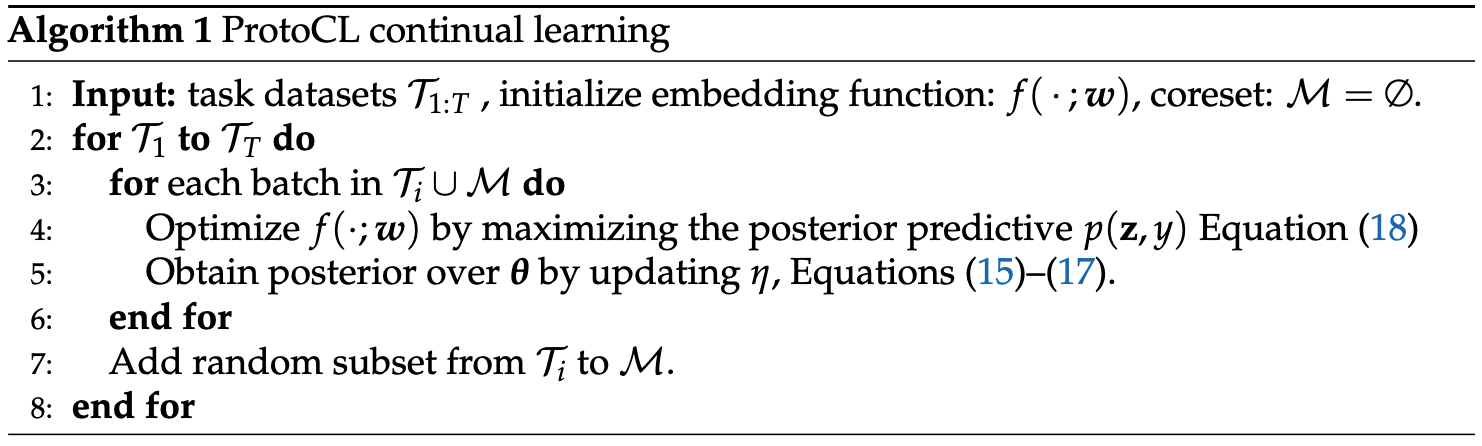
\includegraphics[width=\textwidth]{"images/Algo1.png"}
	\end{figure}
\end{frame}




%%%%%%%%%%%%%%%%%%%%%%%%%%%%%%%
\begin{frame}{ProtoCL Results}
    \begin{figure}
		\centering
		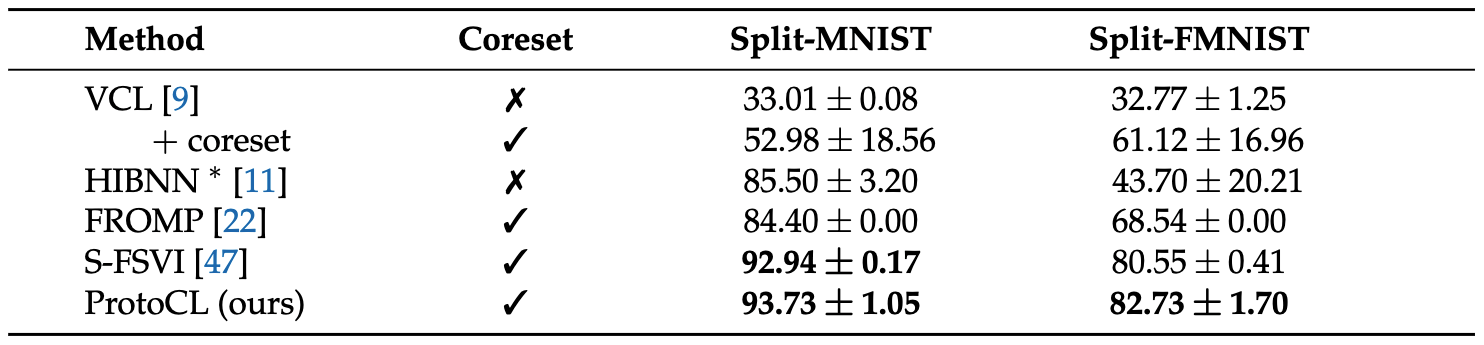
\includegraphics[width=\textwidth]{"images/Table1_pic.png"}
	\end{figure}
 %    \begin{figure}
	% 	\centering
	% 	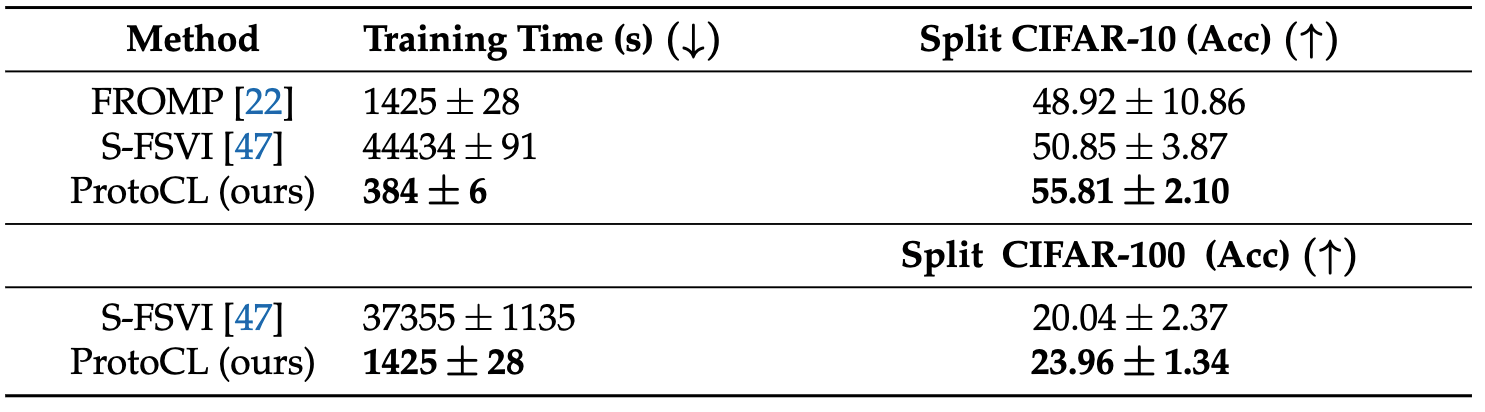
\includegraphics[width=\textwidth]{"images/Table2_pic.png"}
	% \end{figure}
\end{frame}

%%%%%%%%%%%%%%%%%%%%%%%%%%%%%%%
\begin{frame}{ProtoCL Results}
 %    \begin{figure}
	% 	\centering
	% 	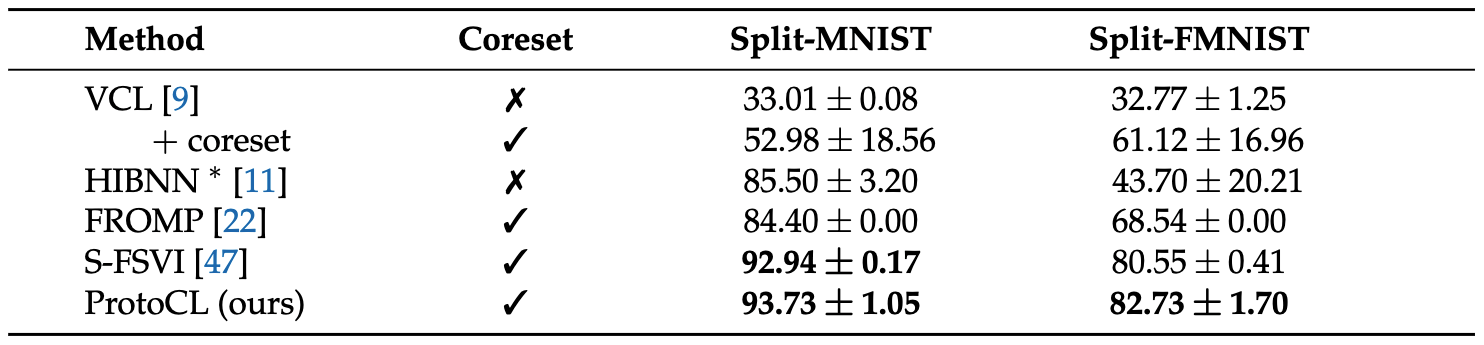
\includegraphics[width=\textwidth]{"images/Table1_pic.png"}
	% \end{figure}
    \begin{figure}
		\centering
		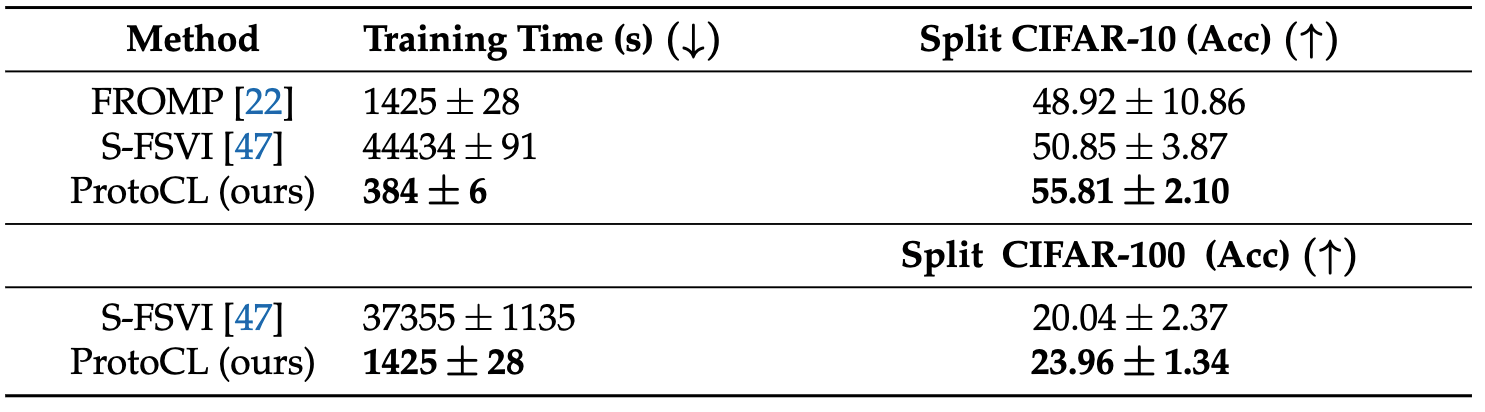
\includegraphics[width=\textwidth]{"images/Table2_pic.png"}
	\end{figure}
\end{frame}

%%%%%%%%%%%%%%%%%%%%%%%%%%%%%%%
\begin{frame}{ProtoCL: Criticisms}
\begin{columns}
    \begin{column}{0.6\textwidth}
        \begin{figure}
		\centering
		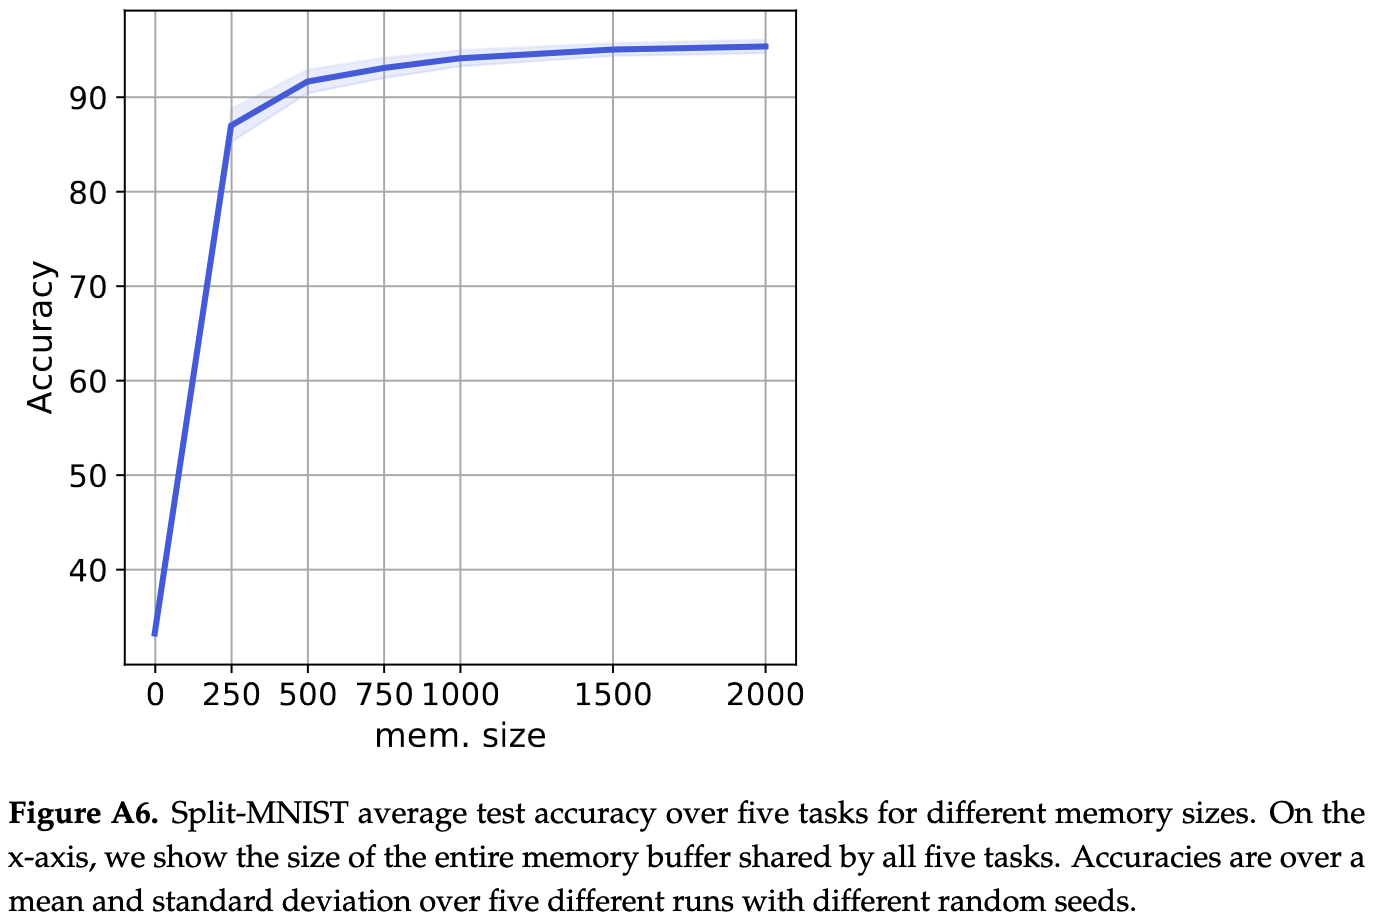
\includegraphics[width=\textwidth]{"images/FigA6_full.png"}
	\end{figure}
    \end{column}
    \begin{column}{0.4\textwidth}
        \begin{itemize}[<+->]
            \item Core set %(seems a bit like cheating but I think there's no way of avoiding the fact that it works and everyone does it)
            \item Heavily dependent on embedding dimension
            \begin{itemize}
                \item (F)MNIST: 128
                \item CIFAR10/100: 32
            \end{itemize}
            %\item ``The stated aim of ProtoCL is not to provide a novel state-of-the-art method for CL, but rather to propose a simple baseline that takes an alternative route than weight-space sequential Bayesian inference.''
        \end{itemize}
    \end{column}
    
    
\end{columns}
    
\end{frame}

%%%%%%%%%%%%%%%%%%%%%%%%%%%%%%%
\begin{frame}{ProtoCL: Criticisms}

    ``\textit{The stated aim of ProtoCL is not to provide a novel state-of-the-art method for CL, but rather to propose a simple baseline that takes an alternative route than weight-space sequential Bayesian inference.}''
    
\end{frame}

% %%%%%%%%%%%%%%%%%%%%%%%%%%%%%%%
% \section{Conclusion}
% \begin{frame}{Conclusion}
% \begin{itemize}[<+->]
%     \item Cool direction
%     \item Increased simplicity compared to VCL (arguably)
%     \item Has it been used since? 
%         \begin{itemize}
%             \item The BNN update theory in this paper is used by \cite{lu_ibcl_2023}, but this doesn't use ProtoCL and doesn't seem massively impressive at a quick glance.
%         \end{itemize}
% \end{itemize}
% \end{frame}

%%%%%%%%%%%%%%%%%%%%%%%%%%%%%%%
\begin{frame}[allowframebreaks]{References}
    \printbibliography
    
\end{frame}


\end{document}